\section{Methodology Descripttion}
\subsection{ETL Data}
\subsubsection{Data Sources}
For the data extraction process, we utilized product reviews and specifications from the \href{https://pricebaba.com/}{pricebaba} website. This site offers a comprehensive range of products, including mobile phones, laptops, televisions, and other electronic devices. For this research, we initially focused exclusively on mobile phone data. The site provides detailed product information and expert reviews, making it a valuable data source for training and evaluating review generation models.
\\\\
The reviews are structured as shown in Figure \ref{fig:pricebaba-review-structure}, Each review includes a detailed description of the product, pros and cons, and descriptions focused on various features such as the camera, battery, screen, etc. Additionally, Figure \ref{fig:pricebaba-spec-structure} shows that the product specifications are structured in tables and sub-tables, facilitating data extraction.
\begin{figure}[H]
    \centering
    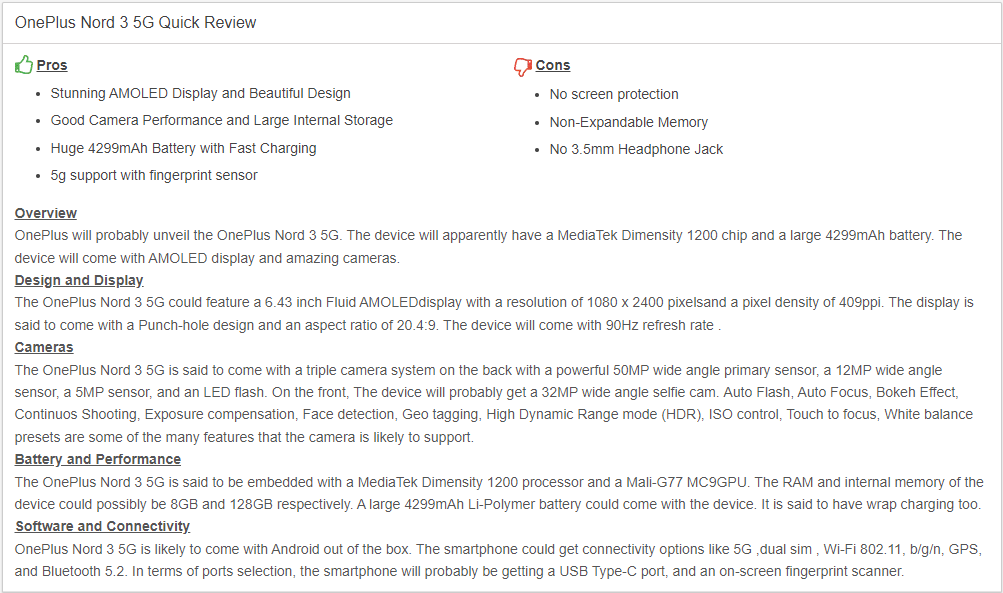
\includegraphics[width=12cm]{images/pricebaba_review_structure.png}
    \caption{pricebaba reviews structure}
    \label{fig:pricebaba-review-structure}
\end{figure}
\begin{figure}[H]
    \centering
    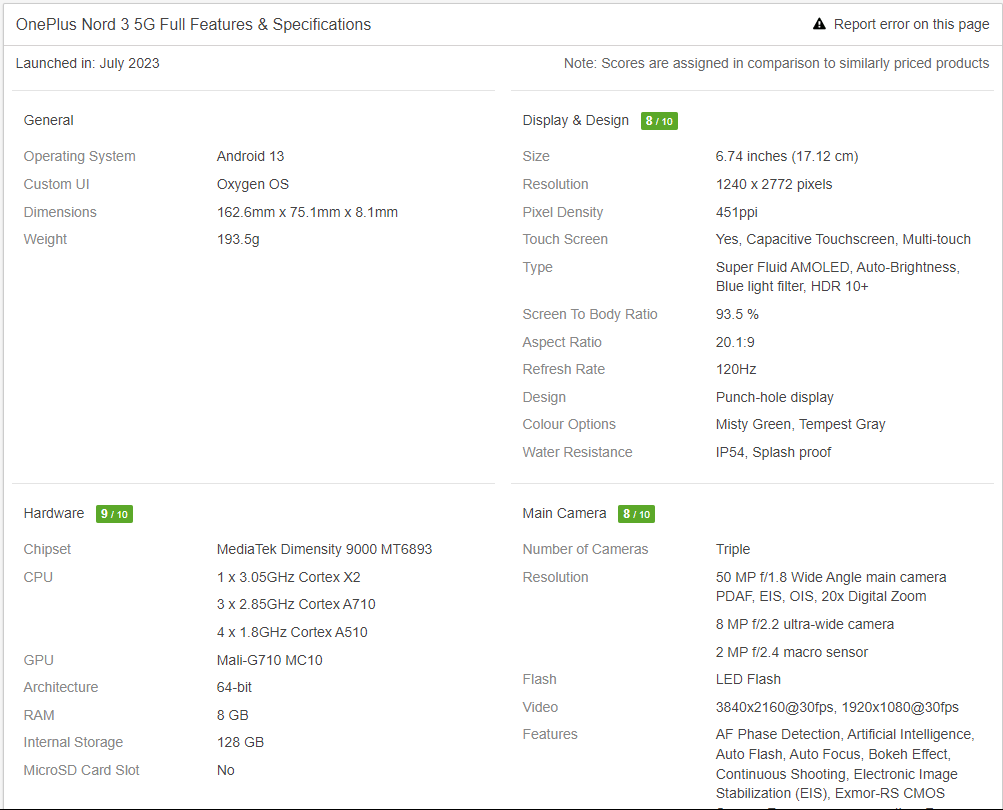
\includegraphics[width=12cm]{images/pricebaba_spec_structure.png}
    \caption{pricebaba specifications structure}
    \label{fig:pricebaba-spec-structure}
\end{figure}
To achieve data extraction, we will use the technique of web scraping, which involves extracting information from web pages and storing it in a database. In this case, we will extract reviews and specifications of mobile phones from the pricebaba website and store them in JSON format for subsequent processing. This process yielded a dataset of reviews and specifications for 7400 mobile phones, serving as the initial database for cleaning and formatting.

\subsubsection{Data Format}
The chosen format for data representation is JSON, as this format allows for structured and easy-to-process data representation. Two JSON files will be used to represent the data: one for the reviews and another for the product specifications. Each JSON file will contain an array of objects, where each object will represent a product along with its respective reviews or specifications. The structure of the JSON files is outlined below:
\newpage
\begin{lstlisting}[style=jsonstyle, frame = single, caption=JSON Data Format Product specification, label=code:json-data-format]
{
    "url": {
        "Launch Date": "Launch Date",
        "General": {
            "subcategories1": [
                "value1"
                ],
            "subcategories2": [
                "value1",
                "value2"
                ],
            ...
        },
        "Characteristic1": {
            "subcategories1": [
                "value1"
                ],
            "subcategories2": [
                "value1",
                "value2"
                ],
            ...
        },
        "Characteristic2": {
            "subcategories1": [
                "value1"
                ],
            "subcategories2": [
                "value1",
                "value2"
                ],
            ...
        },
        ...
    },
}
\end{lstlisting}
\newpage
\begin{lstlisting}[style=jsonstyle, frame = single, caption=JSON Data Format reviews, label=code:json-data-format]
{
    "url": {
        "text": {
            "Characteristic1": ["Description1"],
            "Characteristic2": ["Description2"],
            ...
        },
        "Pros": [
            "Pro 1",
            "Pro 2",
            "Pro 3"
        ],
        "Cons": [
            "Con 1",
            "Con 2",
            "Con 3"
        ]
    },
}
\end{lstlisting}

\subsubsection{Data Cleaning Process}
Once the data has been extracted, a cleaning process is necessary to ensure that the data is coherent and ready for processing by the models. The following cleaning tasks will be performed:

\paragraph{Normalization}
After structuring the data into JSON format, normalization is carried out. This involves evaluating the keys of the objects, cleaning keys that contain spaces, transforming keys, subkeys, and values to lowercase, replacing `\&` with `and`, and reordering keys that include `and` to maintain a logical order. For instance, the key `Display \& Design` was changed to `Design and Display`.

\paragraph{Data Removal}
Once all data is normalized, the process of removing duplicates and unnecessary data begins. This will include deleting reviews that contain no value in the `text` key, specifications that only have the value `General`, or reviews that only contain the value `Overview`. This is because our goal is to conduct detailed product reviews based on their distinct characteristics, rather than in a generalized manner.

\subsubsection{Split data}
Once the data has been cleaned and structured, the dataset is divided into three sets: training, and testing. For this, an 80\% portion will be allocated for training and 20\% for testing. This ensures that the models are trained with a sufficient amount of data and evaluated appropriately.
\\\\
Priority is given to using the most recent product data for the test set to ensure that the models are evaluated with the most current data, thereby preventing the models from encountering similar data within their training slice. For this purpose, the dataset is sorted by the Launch Date key in descending order, and the top 20\% of the data is selected for the test set. This guarantees that the models are evaluated with the most recent data and prevents the models from memorizing the training data.

\subsubsection{Prompt structuration}
Once the JSONs for reviews and specifications have been cleaned, the next step is to structure the instructions that will be used to train the models. These instructions will form the final dataset. For this purpose, instructions with the following structure will be created:
\begin{lstlisting}[style=textstyle, frame = single, caption=Prompt structuration, label=code:prompt-structuration]
"Given following json that contains specifications of a product, generate a review of the key characteristics with json format. Follow the structure on Keys to write the Output: 
### Product: Product for JSON specifications
### Keys: Combination of the keys of the JSON reviews
### Output: reviews for JSON reviews accordingly to the keys"
\end{lstlisting}
it means that instructions will be generated for each permutation of the review keys. For example, if there is a review with the keys Design and Display', Camera', Battery', Performance', Software', i' instructions are chosen from the possible combinations of these keys, where i' is the number of instructions desired to be generated. This approach ensures that the model generates reviews according to the different characteristics of the products. An example of key selection could be that if a product has the keys Design and Display', Camera', Battery', Performance', Software', then the keys Design and Display', Camera' might be selected to generate one instruction, and for another instruction for the same product, the keys Design and Display', Battery' might be selected, and so on.
\\\\
With these combinations of keys for generating instructions, from the original 7,400 data points, 60,700 instructions are obtained that will be used to train the models. These instructions are the final dataset, which is available on \href{https://huggingface.co/datasets/kokujin/json_data_luis}{Hugginface}.

\subsection{Model Fine-Tuning}
\subsubsection{Hyperparameter Selection}
Due to the fact that the Large Language Models (LLMs) to be used are already pretrained, the hyperparameters selected will be those used for the fine-tuning process of the models. Additionally, due to computational limitations, hyperparameters that fit the capabilities of the machine on which the fine-tuning process will be conducted will be selected. For this purpose, the hyperparameters from Table \ref{table:hyperparameters} will be chosen.
\begin{table}[H]
    \centering
    \begin{tabular}{|c|c|}
        \hline
        \textbf{Hyperparameter} & \textbf{Value} \\
        \hline
        Learning Rate & 2e-4 \\
        Batch Size & 2 \\
        Epochs & 1 \\
        max\_grad\_norm & 0.3 \\
        gradient\_accumulation\_steps & 1 \\
        weight\_decay & 0.001 \\
        warmup\_ratio & 0.03 \\
        lr\_scheduler\_type & cosine \\
        optim & adam \\
        max\_seq\_length & 900 \\
        \hline
    \end{tabular}
    \caption{Hyperparameters Selection}
    \label{table:hyperparameters}
\end{table}
The choice of `max\_seq\_length` is based on prior estimation of the average token length of the reviews, which was found to be 900 tokens. To achieve this, it was necessary to iterate through each prompt and use a tokenizer. Furthermore, the `BitsAndBytesConfig` library from Hugging Face's `transformers` has been utilized for model optimization. These additional hyperparameters are shown in Table \ref{table:hyperparameters-bitsandbytes}.
\begin{table}[H]
    \centering
    \begin{tabular}{|c|c|}
        \hline
        \textbf{Hyperparameter} & \textbf{Value} \\
        \hline
        bnb\_4bit\_compute\_dtype & float16 \\
        bnb\_4bit\_quant\_type & nf4 \\
        use\_nested\_quant & False \\
        \hline
    \end{tabular}
    \caption{Hyperparameters Selection BitsAndBytes}
    \label{table:hyperparameters-bitsandbytes}
\end{table}

\subsection{Model Evaluation}
Once the models have been fine-tuned, they are evaluated using the test data. For this purpose, metrics such as BLEU, METEOR, and ROUGE were used. These metrics compare the reviews generated by the models with the actual product reviews, thereby assessing the quality of the reviews produced by the models and determining which model best fits the test data.
\\\\
Additionally, the model's tendency to hallucinate when generating product reviews will be evaluated. This will be achieved through reverse engineering, meaning transforming the reviews back into specifications and comparing them with the actual product specifications. Three aspects will be evaluated as specified in Figure \ref{fig:evaluation-structure}:
\begin{figure}[H]
    \centering
    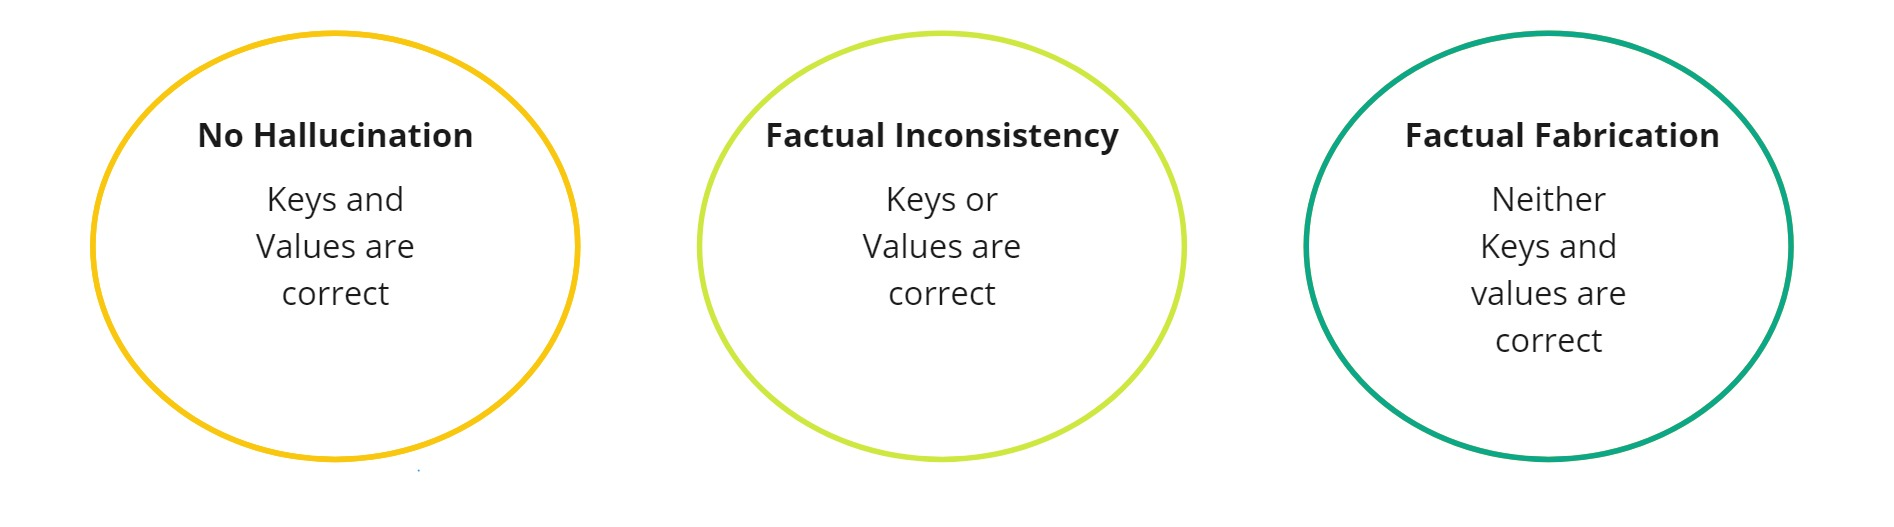
\includegraphics[width=12cm]{images/evaluation_structure.jpg}
    \caption{evaluation structure}
    \label{fig:evaluation-structure}
\end{figure}
The effectiveness of the model's language generation will also be examined to ensure that the text produced is not only accurate but also stylistically consistent with typical user-generated reviews. This helps in enhancing the perceived authenticity of the generated content. Moreover, the response time of the model and its ability to handle large datasets efficiently will also be analyzed, which are crucial for real-world applications where processing speed and scalability are essential.

\subsection{Resume}
This section provides a detailed overview of the methodology used for generating product reviews on e-commerce platforms using Large Language Models (LLMs). It describes the entire process from data collection and preparation, where data was generated from scratch, meticulously cleaned, and structured for further processing.
\\\\
The section continues by detailing the model tuning techniques, including the selection of hyperparameters and optimization methods, tailored to match the computational limits of the hardware. This phase was essential for adapting the models to produce relevant product reviews. The effectiveness of these fine-tuned models was then measured using evaluation metrics such as BLEU, METEOR, and ROUGE to assess the quality of generated reviews against actual product reviews.